\documentclass[
11pt, % The default document font size, options: 10pt, 11pt, 12pt
codirector, % Uncomment to add a codirector to the title page
]{charter} 




% El títulos de la memoria, se usa en la carátula y se puede usar el cualquier lugar del documento con el comando \ttitle
\titulo{Monitoreo de equipos heating
ventilating air conditioned (HVAC) en
laboratorio farmacéutico. } 

% Nombre del posgrado, se usa en la carátula y se puede usar el cualquier lugar del documento con el comando \degreename
%\posgrado{Carrera de Especialización en Sistemas Embebidos} 
\posgrado{Carrera de Especialización en Internet de las Cosas} 
%\posgrado{Carrera de Especialización en Intelegencia Artificial}
%\posgrado{Maestría en Sistemas Embebidos} 
%\posgrado{Maestría en Internet de las cosas}

% Tu nombre, se puede usar el cualquier lugar del documento con el comando \authorname
\autor{Federico Manuel Suarez Paris} 

% El nombre del director y co-director, se puede usar el cualquier lugar del documento con el comando \supname y \cosupname y \pertesupname y \pertecosupname
\director{A definir}
\pertenenciaDirector{A definir} 
% FIXME:NO IMPLEMENTADO EL CODIRECTOR ni su pertenencia
%
\codirector{A DEFINIR} % para que aparezca en la portada se debe descomentar la opción codirector en el documentclass
\pertenenciaCoDirector{FIUBA}

% Nombre del cliente, quien va a aprobar los resultados del proyecto, se puede usar con el comando \clientename y \empclientename
\cliente{Ing. Pablo Covello}
\empresaCliente{Laboratorio Baliarda S.A.}

% Nombre y pertenencia de los jurados, se pueden usar el cualquier lugar del documento con el comando \jurunoname, \jurdosname y \jurtresname y \perteunoname, \pertedosname y \pertetresname.
\juradoUno{Nombre y Apellido (1)}
\pertenenciaJurUno{pertenencia (1)} 
\juradoDos{Nombre y Apellido (2)}
\pertenenciaJurDos{pertenencia (2)}
\juradoTres{Nombre y Apellido (3)}
\pertenenciaJurTres{pertenencia (3)}
 
\fechaINICIO{25 de abril de 2023}		%Fecha de inicio de la cursada de GdP \fechaInicioName
\fechaFINALPlan{26 de junio de 2023} 	%Fecha de final de cursada de GdP
\fechaFINALTrabajo{18 de diciembre de 2023}	%Fecha de defensa pública del trabajo final


\begin{document}

\maketitle
\thispagestyle{empty}
\pagebreak


\thispagestyle{empty}
{\setlength{\parskip}{0pt}
\tableofcontents{}
}
\pagebreak


\section*{Registros de cambios}
\label{sec:registro}


\begin{table}[ht]
\label{tab:registro}
\centering
\begin{tabularx}{\linewidth}{@{}|c|X|c|@{}}
\hline
\rowcolor[HTML]{C0C0C0} 
Revisión & \multicolumn{1}{c|}{\cellcolor[HTML]{C0C0C0}Detalles de los cambios realizados} & Fecha      \\ \hline
1      & Con avances hasta el punto 5                                 &\fechaInicioName 
\\ \hline
2      & Se completa hasta el punto 7 inclusive                 & 16 de mayo de 2023 \\ \hline
%2      & Se completa hasta el punto 7 inclusive
%		  Se puede agregar algo más \newline
%		  En distintas líneas \newline
%		  Así                                                    & dd/mm/aaaa \\ \hline
%3      & Se completa hasta el punto 11 inclusive                & dd/mm/aaaa \\ \hline
%4      & Se completa el plan	                                 & dd/mm/aaaa \\ \hline
\end{tabularx}
\end{table}

\pagebreak



\section*{Acta de constitución del proyecto}
\label{sec:acta}

\begin{flushright}
Buenos Aires, \fechaInicioName
\end{flushright}

\vspace{2cm}

Por medio de la presente se acuerda con el Lic. \authorname\hspace{1px} que su Trabajo Final de la \degreename\hspace{1px} se titulará ``\ttitle'', consistirá esencialmente en {la implementación de un prototipo de un sistema de monitoreo de equipos de HVAC en un laboratorio farmaceutico}, y tendrá un presupuesto preliminar estimado de {600} h de trabajo y {A DEFINIR}, con fecha de inicio \fechaInicioName\hspace{1px} y fecha de presentación pública \fechaFinalName.

Se adjunta a esta acta la planificación inicial.

\vfill

% Esta parte se construye sola con la información que hayan cargado en el preámbulo del documento y no debe modificarla
\begin{table}[ht]
\centering
\begin{tabular}{ccc}
\begin{tabular}[c]{@{}c@{}}Dr. Ing. Ariel Lutenberg \\ Director posgrado FIUBA\end{tabular} & \hspace{2cm} & \begin{tabular}[c]{@{}c@{}}\clientename \\ \empclientename \end{tabular} \vspace{2.5cm} \\ 
\multicolumn{3}{c}{\begin{tabular}[c]{@{}c@{}} \supname \\ Director del Trabajo Final\end{tabular}} \vspace{2.5cm} \\
%\begin{tabular}[c]{@{}c@{}}\jurunoname \\ Jurado del Trabajo Final\end{tabular}     &  & \begin{tabular}[c]{@{}c@{}}\jurdosname\\ Jurado del Trabajo Final\end{tabular}  \vspace{2.5cm}  \\
%\multicolumn{3}{c}{\begin{tabular}[c]{@{}c@{}} \jurtresname\\ Jurado del Trabajo Final\end{tabular}} \vspace{.5cm}                                                                     
\end{tabular}
\end{table}




\section{1. Descripción técnica-conceptual del proyecto a realizar}
\label{sec:descripcion}


% El bloque "consigna" se usa para poner texto en rojo y dar una pequeña ayuda sobre cómo completar la sección. En cada entrega parcial deben eliminar los comandos begin y end del bloque consigna de las secciones que hayan completado.
En en la planta Santa Cruz de los Laboratorios Baliarda S.A., se dispone de 16 equipos de HVAC que se desean monitorear.\par 
9 de estos equipos son del tipo \textit{Rooftop} y 7 son unidades manejadoras de aire.
 En los días muy cálidos o muy fríos, estos equipos, tienden a salir de servicio por el accionamiento de alguna de sus seguridades. \par 
Por ejemplo, en los días muy calurosos, con temperaturas superiores a 35°, puede ser que se accione un presostato de alta presión de gas de algún compresor (Gas Freon, R22, R407, R410). \par 
En cambio, en los días muy fríos, con temperaturas inferiores a 6°, puede ser que se accione un presostato de baja presión de gas de algún compresor (Gas Freon, R22, R407, R410). \par 
 Estas situaciones, en los equipos, se detectan en los sectores asociados, a los 30 minutos o hasta una hora después de que ocurrió el evento dentro del HVAC. \par 
Como consecuencia, los sectores que dependen de los equipos en falla, deben detener la producción hasta normalizar la temperatura de trabajo del sector. \par 
 Lo que propone este proyecto, es tener una rápida respuesta ante un evento de falla en los equipos de HVAC para así minimizar las detenciones de los sectores productivos por exceso o falta de temperatura. \par 
Por otro lado, se busca tener un historial para evaluar el comportamiento de los equipos durante el día y la noche.\par 
Este proyecto estará a un repositorio* donde, el código fuente, podrá ser implementado en cualquier empresa o institución que lo requiera con la salvedad de que si el sistema es utilizado fuera de la empresa Baliarda S.A., no se podrán utilizar nombres de equipos, divulgar procesos o cualquiera otra información confidencial de Baliarda S.A. \par 
Para el funcionamiento del sistema se utilizará un microcontrolador ESP32 en cada unidad a monitorear. Se diseñará una plaqueta donde tendrá montado el ESP32, la fuente de alimentación y 4 relays de 24 VCC que serán los encargados de enviar la señal de los estados al microcontrolador. Por otro lado, se diseñará un sistema de UPS*, en caso de corte de energía eléctrica, con 1 hora de autonomía.\par 
Cada equipo tendrá un microcontrolador que reportará los datos a una base de datos relacional de Postgres en un servidor local.\par 
Desde cualquier PC, dentro de la red del laboratorio y por exigencia de Baliarda S.A., se accederá a través de una página web (API) mostrando todos los HVAC y sus estados.\par 
El ingreso se realizará mediante usuario y contraseña 2 (dos) niveles de acceso (Supervisor y Operador)
El Operador, podrá ver las temperaturas, los estados y los históricos.
El Supervisor tendrá el control total del sistema.
La Clave de los usuarios expirara, mínimamente, cada 3 meses.
Cada imagen tendrá un link donde se redirigirá al microcontrolador asociado a ese equipo.
Dentro de cada imagen de HVAC se podrán realizar las siguientes operaciones:
\begin{itemize}
\item Histórico de temperaturas y estados.
\item Configuración de correos electrónicos para enviar alarmas.
\item Mensajes de las alarmas.
\item Configuración de Wi-Fi.
\item Potencia de señal de Wi-Fi.
\item SetPoint de temperatura.
\end{itemize}
La comunicación de todo el sistema deberá ser vía Wi-Fi. \par 
La placa con el microcontrolador estará dentro de una caja plástica fabricada con materiales que no propaguen la llama. Esta caja, tendrá una señalización donde indique el estado de las entradas digitales, conexión con una red Wi-Fi y tensión del equipo. \par 
Se fabricará un prototipo con su \textit{firmware} para 1 ESP32 con su placa y su caja, la programación y la visualización de los equipos HVAC.\par 
En el siguiente diagrama se muestra como debe funcionar el sistema.\par


\begin{figure}[H]
\centering 
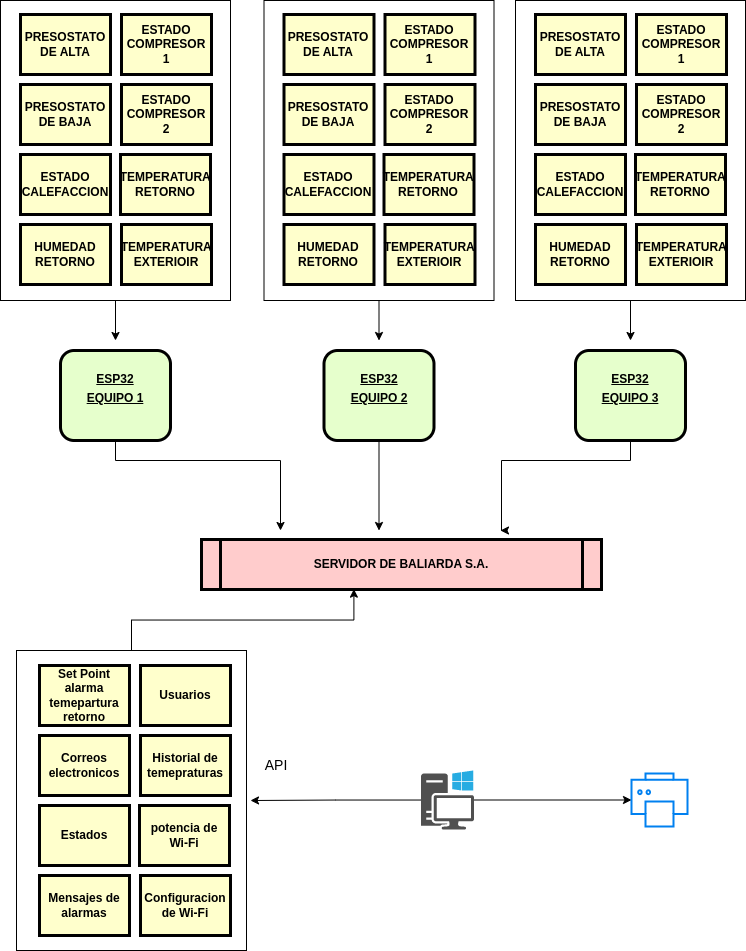
\includegraphics[width=1.1\textwidth]{./Figuras/DIAGRAMA_1.png}
\caption{Diagrama en bloqes del sistema}
\label{fig:diagBloques}
\end{figure}

\vspace{25px}





GLOSARIO:
*UPS: Uninterruptible Power System.
*SetPoint: Punto de configuración.
*Repositorio: espacio centralizado donde se guardan trabajos científicos, archivos, etc.



\section{2. Identificación y análisis de los interesados}
\label{sec:interesados}


\begin{table}[ht]
%\caption{Identificación de los interesados}
%\label{tab:interesados}
\begin{tabularx}{\linewidth}{@{}|l|X|X|l|@{}}
\hline
\rowcolor[HTML]{C0C0C0} 
Rol           & Nombre y Apellido & Organización 	& Puesto 	\\ \hline
Cliente       & \clientename      &\empclientename	&Gerente de ingenieria \\ \hline
Impulsor      & Ing.Juan Cendron  &Balairda S.A.    & Jefe de mantenimiento \\ \hline
Responsable   & \authorname       & FIUBA        	& Alumno 	\\ \hline
Orientador    & \supname	      & \pertesupname 	& Director Trabajo final \\ \hline
Usuario final & \empclientename   &\empclientename  &      -  	\\ \hline
\end{tabularx}
\end{table}

\section{3. Propósito del proyecto}
\label{sec:proposito}

El proposito del presente proyecto es mejorar el control de los equipos HVAC de la planta.


\section{4. Alcance del proyecto}
\label{sec:alcance}


El alcance de este proyecto será:
\begin{itemize}
\item La creación un software de gestión de los HVAC.
\item La creación del \textit{firmware} para el esp32.
\item La fabricación de prototipo.
\item 5 horas de asistencia técnica in situ.
\item 5 horas de asistencia técnica a distancia. 
\end{itemize}
El presente proyecto no incluye:
\begin{itemize}
\item La fabricación de los dispositivos restantes.
\item La instalación.
\item La puesta en marcha. 
\end{itemize}




\section{5. Supuestos del proyecto}
\label{sec:supuestos}

Para el desarrollo del presente proyecto se supone que:




\begin{itemize}
	\item La Gerencia, Jefatura y Supervision de mantenimiento tendra un mejor control de los equipos HVAC de la planta.
	\item El departamento de Garantia de calidad tendra mas datos para invertigar desvios producto de la falla de los HVAC.
	\item Ajustar los mantenimientos preventivos de los equipos de HVAC.
	\item Optimizar el uso de los HVAC.
	\item Advertir a tiempo la falla de un equipo 
\end{itemize}

\section{6. Requerimientos}
\label{sec:requerimientos}

\begin{enumerate}
	\item Requerimientos funcionales
		\begin{enumerate}
			\item El sistema debe poder manejar la visualizacion de del estado, las larmas y las temperaturas de los 16 equipos de aire acondicionado
			\item los ESP32 de cada equipo se debe conectar con un equipo o servidor central para lograr almacenar los datos recolectados en una base de datos.
			\item El usuario debe poder recolectar los datos guardados en la base de datos. Debe poder buscar datos por fecha y debera poder imprimir lo recolectado.
		\end{enumerate}
	\item Requerimientos de documentación
		\begin{enumerate}
			\item Manual de programacion del \textit {firmware} del ESP32.
			\item Manual de instalacion del ESP32.
			\item Manual de uso del ESP32.
			\item Manual de configuracion de la API.
			\item Manual de configuracion de la base de datos.
			\item Manual de uso de la API.
			
			
		\end{enumerate}
	\item Requerimiento de testing del \textit{firmaware} de ESP32.
	\item Requerimientos de testing de la interfaz grafica.
	\item Requerimiento de testing de la seguridad del sistema.
\end{enumerate}

\section{7. Historias de usuarios (\textit{Product backlog})}
\label{sec:backlog}
Roles
Operador:
\begin{itemize}
 \item Podrá ver todos los datos de la API. 
 \item Podrá descargar históricos de la base de datos.
 \item Podrá buscar datos.
 \item Podrá imprimir datos seleccionados.
\end{itemize}
Supervisor:
\begin{itemize}
\item Podrá cargar los correos electronicos de los destinatarios de las alarmas.
\item Podrá crear usuarios y la primera clave con su tiempo de expiración.
\item Podrá configurar los setpoint de las alarmas.
\item Podrá dar el alta/baja de dispositivos.
\item Podrá asignar las direcciones IP de tlos dispositivos y base de datos.
\end{itemize}


Para asignar la ponderación a los \textit {story points} se han definido los siguientes criterios basados en la dificultad , complejidad y riesgo del trabajo a realizar. \par
Dificultad del trabajo a realizar:
\begin{itemize}
 \item Bajo  = 1 
 \item Medio = 3
 \item Alto = 5
\end{itemize}

Complejidad del trabajo a realizar:
\begin{itemize}
 \item Bajo  = 1 
 \item Medio = 3
 \item Alto = 5
\end{itemize}

Riesgo del trabajo a realizar:

\begin{itemize}
 \item Bajo  = 1 
 \item Medio = 3
 \item Alto = 5
\end{itemize}

Historias de usuario 1: Como desarrollador quiero diseñar un sistema de monitoreo de equipos de HVAC en una planta farmacéutica.

\begin{itemize}
 \item Dificultad alta (5): Porque este sistema conlleva diseñar varios software y \textit {firmware}.
 \item Complejidad media (3): Porque se requiere conocimientos de diseños de la API, Base de datos y programación de ESP32.
 \item Riesgo medio (3): Durante el desarrollo y la implementación pueden surgir varios inconvenientes que se solucionaran en el momento que ocurran.
\end{itemize}
\textit {Story points} 13  (5 + 3 + 3 = 11 => 13) La ponderación es de 11 puntos. Al buscarlo en la serie de Fibonacci la ponderación es de 13 puntos.

Historia de usuario 2: Como usuario quiero monitorear los equipos de HVAC desde una pc.


\begin{itemize}
 \item Dificultad bajo (1): El sistema me permite visualizar todos los datos de los equipos HVAC.
 \item Complejidad media (3): Se requieren conocimientos de los equipos controlados para interpretar los datos recolectados por el sistema.
 \item Riesgo bajo (1): Leer los datos recolectados no presenta ningún problema al sistema y a las instalaciones.
\end{itemize}

\textit {Story points} 5 (1 + 3 + 1 = 5 => 5) La ponderación es  de 5 puntos. Al buscarlo en la serie de Fibonacci el valor tambien es de 5 puntos.

Historias de usuario 3: Como usuario quiero ajustar los setpoints de control de los HVAC.

\begin{itemize}
 \item Dificultad alta (5): El sistema no me permite controlar los HVAC. Se requiere otro \textit {firmware} para el ESP32. 
 \item Complejidad alta (5): Se requiere realizar un nuevo \textit {firmware}  para el ESP32.
 \item Riesgo Alto (5): Para controlar los equipos HVAC se requiere una modificación en el codigo de la API.
\end{itemize}
\textit {Story points} 15 (5 + 5 + 5 = 15 => 21) La ponderación es  de 15 puntos. Al buscarlo en la serie de Fibonacci el valor es de 21 puntos.

\section{8. Entregables principales del proyecto}
\label{sec:entregables}


Los entregables del proyecto son:

\begin{itemize}
	\item Manual de uso
	\item Diagrama de circuitos esquemáticos
	\item Código fuente del \textit{firmware} del ESP32.
	\item Código fuente de la API.
	\item Código fuente de la base de datos.
	\item Diagrama de instalación
	\item Informe final
\end{itemize}



\section{9. Desglose del trabajo en tareas}
\label{sec:wbs}

\begin{consigna}{red}
El WBS debe tener relación directa o indirecta con los requerimientos.  Son todas las actividades que se harán en el proyecto para dar cumplimiento a los requerimientos. Se recomienda mostrar el WBS mediante una lista indexada:

\begin{enumerate}
\item Grupo de tareas 1
	\begin{enumerate}
	\item Tarea 1 (tantas h)
	\item Tarea 2 (tantas hs)
	\item Tarea 3 (tantas h)
	\end{enumerate}
\item Grupo de tareas 2
	\begin{enumerate}
	\item Tarea 1 (tantas h)
	\item Tarea 2 (tantas h)
	\item Tarea 3 (tantas h)
	\end{enumerate}
\item Grupo de tareas 3
	\begin{enumerate}
	\item Tarea 1 (tantas h)
	\item Tarea 2 (tantas h)
	\item Tarea 3 (tantas h)
	\item Tarea 4 (tantas h)
	\item Tarea 5 (tantas h)
	\end{enumerate}
\end{enumerate}

Cantidad total de horas: (tantas h)

Se recomienda que no haya ninguna tarea que lleve más de 40 h. 

\end{consigna}

\section{10. Diagrama de Activity On Node}
\label{sec:AoN}

\begin{consigna}{red}
Armar el AoN a partir del WBS definido en la etapa anterior. 

%La figura \ref{fig:AoN} fue elaborada con el paquete latex tikz y pueden consultar la siguiente referencia \textit{online}:

%\url{https://www.overleaf.com/learn/latex/LaTeX_Graphics_using_TikZ:_A_Tutorial_for_Beginners_(Part_3)\%E2\%80\%94Creating_Flowcharts}

\end{consigna}

\begin{figure}[htpb]
\centering 
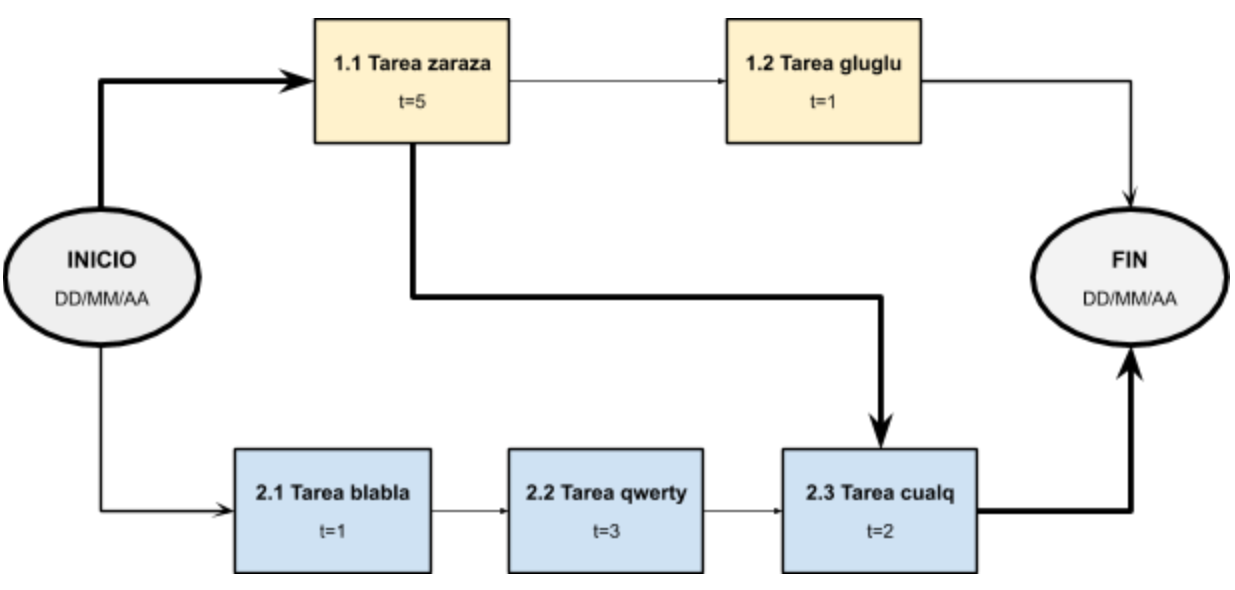
\includegraphics[width=.8\textwidth]{./Figuras/AoN.png}
\caption{Diagrama de \textit{Activity on Node}.}
\label{fig:AoN}
\end{figure}

Indicar claramente en qué unidades están expresados los tiempos.
De ser necesario indicar los caminos semicríticos y analizar sus tiempos mediante un cuadro.
Es recomendable usar colores y un cuadro indicativo describiendo qué representa cada color, como se muestra en el siguiente ejemplo:



\section{11. Diagrama de Gantt}
\label{sec:gantt}

\begin{consigna}{red}

Existen muchos programas y recursos \textit{online} para hacer diagramas de Gantt, entre los cuales destacamos:

\begin{itemize}
\item Planner
\item GanttProject
\item Trello + \textit{plugins}. En el siguiente link hay un tutorial oficial: \\ \url{https://blog.trello.com/es/diagrama-de-gantt-de-un-proyecto}
\item Creately, herramienta online colaborativa. \\\url{https://creately.com/diagram/example/ieb3p3ml/LaTeX}
\item Se puede hacer en latex con el paquete \textit{pgfgantt}\\ \url{http://ctan.dcc.uchile.cl/graphics/pgf/contrib/pgfgantt/pgfgantt.pdf}
\end{itemize}

Pegar acá una captura de pantalla del diagrama de Gantt, cuidando que la letra sea suficientemente grande como para ser legible. 
Si el diagrama queda demasiado ancho, se puede pegar primero la ``tabla'' del Gantt y luego pegar la parte del diagrama de barras del diagrama de Gantt.

Configurar el software para que en la parte de la tabla muestre los códigos del EDT (WBS).\\
Configurar el software para que al lado de cada barra muestre el nombre de cada tarea.\\
Revisar que la fecha de finalización coincida con lo indicado en el Acta Constitutiva.

En la figura \ref{fig:gantt}, se muestra un ejemplo de diagrama de Gantt realizado con el paquete de \textit{pgfgantt}. En la plantilla pueden ver el código que lo genera y usarlo de base para construir el propio.

\begin{figure}[htbp]
\begin{center}
\begin{ganttchart}{1}{12}
  \gantttitle{2020}{12} \\
  \gantttitlelist{1,...,12}{1} \\
  \ganttgroup{Group 1}{1}{7} \\
  \ganttbar{Task 1}{1}{2} \\
  \ganttlinkedbar{Task 2}{3}{7} \ganttnewline
  \ganttmilestone{Milestone o hito}{7} \ganttnewline
  \ganttbar{Final Task}{8}{12}
  \ganttlink{elem2}{elem3}
  \ganttlink{elem3}{elem4}
\end{ganttchart}
\end{center}
\caption{Diagrama de Gantt de ejemplo}
\label{fig:gantt}
\end{figure}


\begin{landscape}
\begin{figure}[htpb]
\centering 
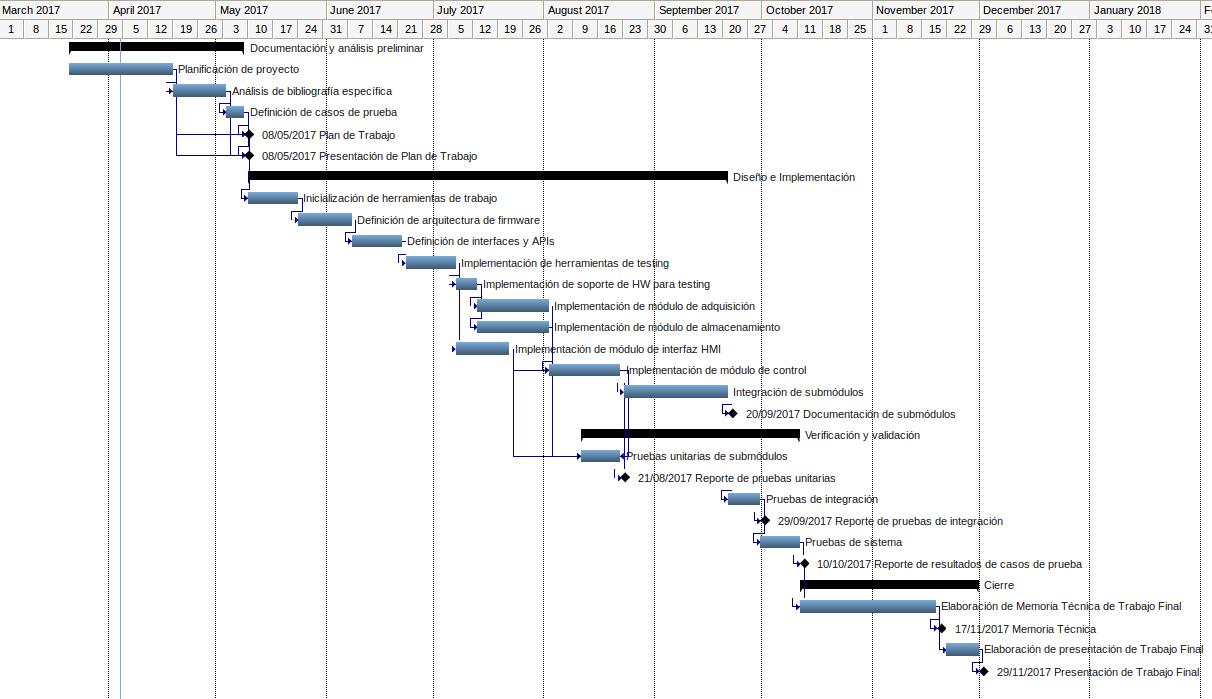
\includegraphics[height=.85\textheight]{./Figuras/Gantt-2.png}
\caption{Ejemplo de diagrama de Gantt rotado}
\label{fig:diagGantt}
\end{figure}

\end{landscape}

\end{consigna}


\section{12. Presupuesto detallado del proyecto}
\label{sec:presupuesto}

\begin{consigna}{red}
Si el proyecto es complejo entonces separarlo en partes:
\begin{itemize}
	\item Un total global, indicando el subtotal acumulado por cada una de las áreas.
	\item El desglose detallado del subtotal de cada una de las áreas.
\end{itemize}

IMPORTANTE: No olvidarse de considerar los COSTOS INDIRECTOS.

\end{consigna}

\begin{table}[htpb]
\centering
\begin{tabularx}{\linewidth}{@{}|X|c|r|r|@{}}
\hline
\rowcolor[HTML]{C0C0C0} 
\multicolumn{4}{|c|}{\cellcolor[HTML]{C0C0C0}COSTOS DIRECTOS} \\ \hline
\rowcolor[HTML]{C0C0C0} 
Descripción &
  \multicolumn{1}{c|}{\cellcolor[HTML]{C0C0C0}Cantidad} &
  \multicolumn{1}{c|}{\cellcolor[HTML]{C0C0C0}Valor unitario} &
  \multicolumn{1}{c|}{\cellcolor[HTML]{C0C0C0}Valor total} \\ \hline
 &
  \multicolumn{1}{c|}{} &
  \multicolumn{1}{c|}{} &
  \multicolumn{1}{c|}{} \\ \hline
 &
  \multicolumn{1}{c|}{} &
  \multicolumn{1}{c|}{} &
  \multicolumn{1}{c|}{} \\ \hline
\multicolumn{1}{|l|}{} &
   &
   &
   \\ \hline
\multicolumn{1}{|l|}{} &
   &
   &
   \\ \hline
\multicolumn{3}{|c|}{SUBTOTAL} &
  \multicolumn{1}{c|}{} \\ \hline
\rowcolor[HTML]{C0C0C0} 
\multicolumn{4}{|c|}{\cellcolor[HTML]{C0C0C0}COSTOS INDIRECTOS} \\ \hline
\rowcolor[HTML]{C0C0C0} 
Descripción &
  \multicolumn{1}{c|}{\cellcolor[HTML]{C0C0C0}Cantidad} &
  \multicolumn{1}{c|}{\cellcolor[HTML]{C0C0C0}Valor unitario} &
  \multicolumn{1}{c|}{\cellcolor[HTML]{C0C0C0}Valor total} \\ \hline
\multicolumn{1}{|l|}{} &
   &
   &
   \\ \hline
\multicolumn{1}{|l|}{} &
   &
   &
   \\ \hline
\multicolumn{1}{|l|}{} &
   &
   &
   \\ \hline
\multicolumn{3}{|c|}{SUBTOTAL} &
  \multicolumn{1}{c|}{} \\ \hline
\rowcolor[HTML]{C0C0C0}
\multicolumn{3}{|c|}{TOTAL} &
   \\ \hline
\end{tabularx}%
\end{table}


\section{13. Gestión de riesgos}
\label{sec:riesgos}

\begin{consigna}{red}
a) Identificación de los riesgos (al menos cinco) y estimación de sus consecuencias:
 
Riesgo 1: detallar el riesgo (riesgo es algo que si ocurre altera los planes previstos de forma negativa)
\begin{itemize}
	\item Severidad (S): mientras más severo, más alto es el número (usar números del 1 al 10).\\
	Justificar el motivo por el cual se asigna determinado número de severidad (S).
	\item Probabilidad de ocurrencia (O): mientras más probable, más alto es el número (usar del 1 al 10).\\
	Justificar el motivo por el cual se asigna determinado número de (O). 
\end{itemize}   

Riesgo 2:
\begin{itemize}
	\item Severidad (S): 
	\item Ocurrencia (O):
\end{itemize}

Riesgo 3:
\begin{itemize}
	\item Severidad (S): 
	\item Ocurrencia (O):
\end{itemize}


b) Tabla de gestión de riesgos:      (El RPN se calcula como RPN=SxO)

\begin{table}[htpb]
\centering
\begin{tabularx}{\linewidth}{@{}|X|c|c|c|c|c|c|@{}}
\hline
\rowcolor[HTML]{C0C0C0} 
Riesgo & S & O & RPN & S* & O* & RPN* \\ \hline
       &   &   &     &    &    &      \\ \hline
       &   &   &     &    &    &      \\ \hline
       &   &   &     &    &    &      \\ \hline
       &   &   &     &    &    &      \\ \hline
       &   &   &     &    &    &      \\ \hline
\end{tabularx}%
\end{table}

Criterio adoptado: 
Se tomarán medidas de mitigación en los riesgos cuyos números de RPN sean mayores a...

Nota: los valores marcados con (*) en la tabla corresponden luego de haber aplicado la mitigación.

c) Plan de mitigación de los riesgos que originalmente excedían el RPN máximo establecido:
 
Riesgo 1: plan de mitigación (si por el RPN fuera necesario elaborar un plan de mitigación).
  Nueva asignación de S y O, con su respectiva justificación:
  - Severidad (S): mientras más severo, más alto es el número (usar números del 1 al 10).
          Justificar el motivo por el cual se asigna determinado número de severidad (S).
  - Probabilidad de ocurrencia (O): mientras más probable, más alto es el número (usar del 1 al 10).
          Justificar el motivo por el cual se asigna determinado número de (O).

Riesgo 2: plan de mitigación (si por el RPN fuera necesario elaborar un plan de mitigación).
 
Riesgo 3: plan de mitigación (si por el RPN fuera necesario elaborar un plan de mitigación).

\end{consigna}


\section{14. Gestión de la calidad}
\label{sec:calidad}

\begin{consigna}{red}
Elija al menos diez requerientos que a su criterio sean los más importantes/críticos/que aportan más valor y para cada uno de ellos indique las acciones de verificación y validación que permitan asegurar su cumplimiento.

\begin{itemize} 
\item Req \#1: copiar acá el requerimiento.

\begin{itemize}
	\item Verificación para confirmar si se cumplió con lo requerido antes de mostrar el sistema al cliente. Detallar 
	\item Validación con el cliente para confirmar que está de acuerdo en que se cumplió con lo requerido. Detallar  
\end{itemize}

\end{itemize}

Tener en cuenta que en este contexto se pueden mencionar simulaciones, cálculos, revisión de hojas de datos, consulta con expertos, mediciones, etc.  Las acciones de verificación suelen considerar al entregable como ``caja blanca'', es decir se conoce en profundidad su funcionamiento interno.  En cambio, las acciones de validación suelen considerar al entregable como ``caja negra'', es decir, que no se conocen los detalles de su funcionamiento interno.

\end{consigna}

\section{15. Procesos de cierre}    
\label{sec:cierre}

\begin{consigna}{red}
Establecer las pautas de trabajo para realizar una reunión final de evaluación del proyecto, tal que contemple las siguientes actividades:

\begin{itemize}
	\item Pautas de trabajo que se seguirán para analizar si se respetó el Plan de Proyecto original:
	 - Indicar quién se ocupará de hacer esto y cuál será el procedimiento a aplicar. 
	\item Identificación de las técnicas y procedimientos útiles e inútiles que se emplearon, y los problemas que surgieron y cómo se solucionaron:
	 - Indicar quién se ocupará de hacer esto y cuál será el procedimiento para dejar registro.
	\item Indicar quién organizará el acto de agradecimiento a todos los interesados, y en especial al equipo de trabajo y colaboradores:
	  - Indicar esto y quién financiará los gastos correspondientes.
\end{itemize}

\end{consigna}


\end{document}
